% methodsandresults.tex

\begin{figure}
\setlength{\abovecaptionskip}{0pt}
\setlength{\belowcaptionskip}{0pt}
\centering
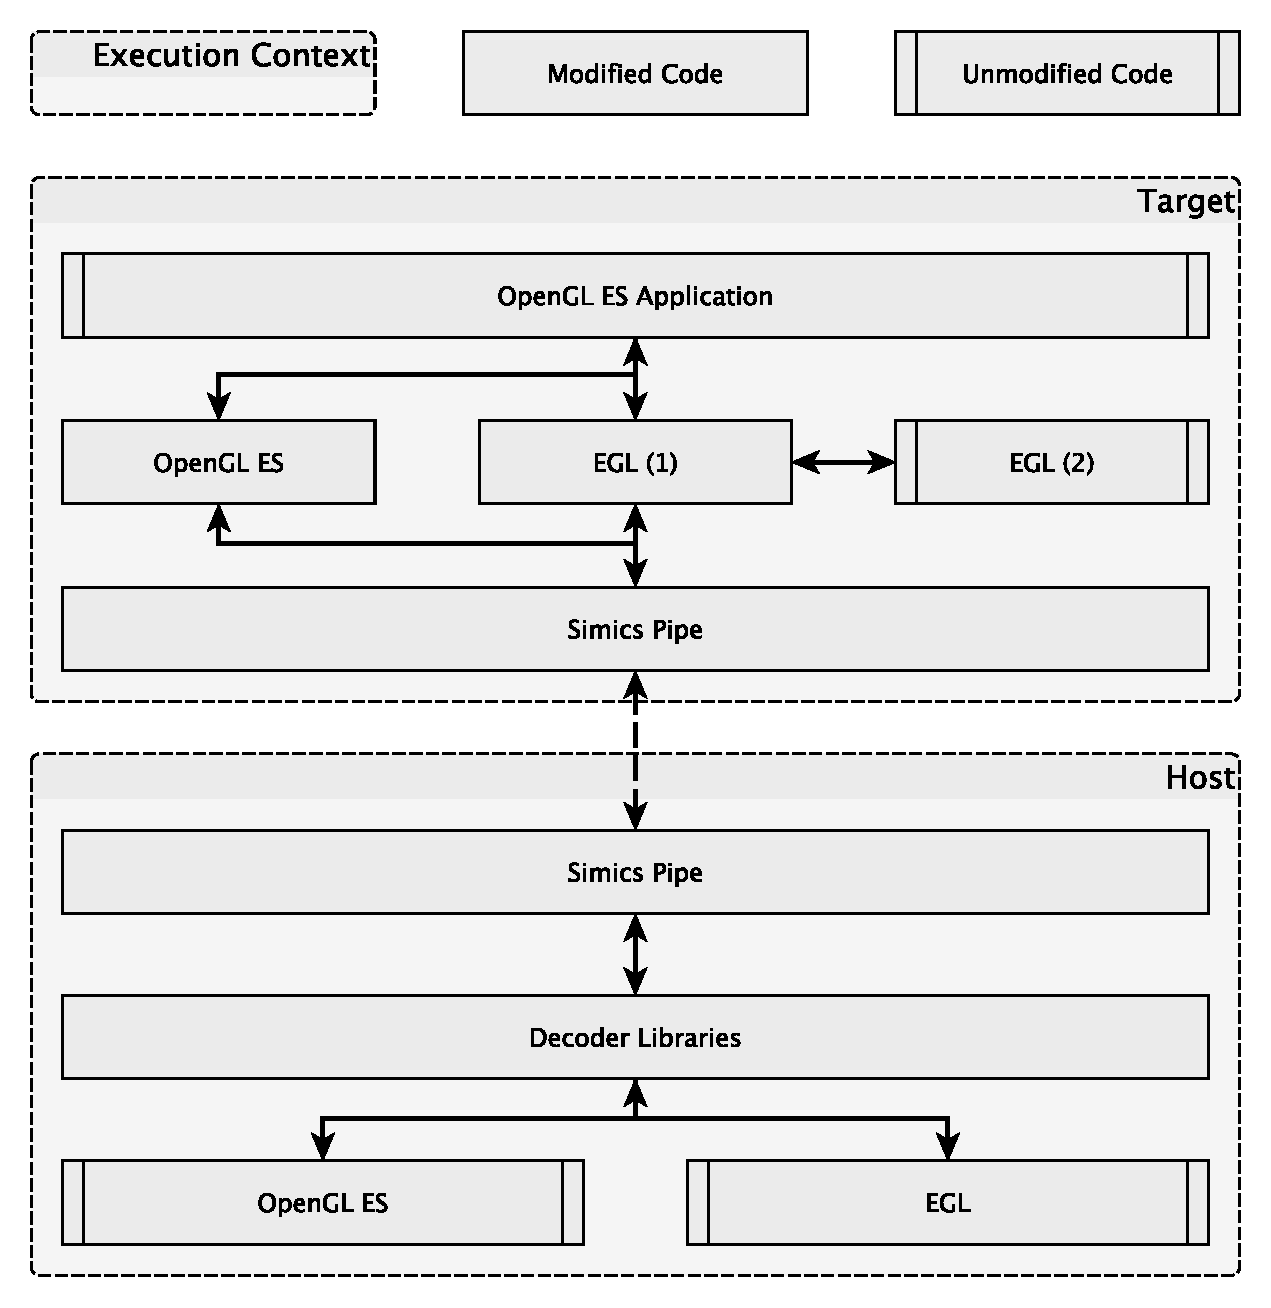
\includegraphics[width=\linewidth]{img/yedoverview.pdf}
\caption{Overview of paravirtualized graphics in Simics.}
\label{fig:overview}
\end{figure}

% Methods and Results
\section{Methods and Results}
\label{sec:methodsandresults}
OpenGL paravirtualization in Simics encompasses three overall components, being the target system libraries, the host system libraries, and a communications channel between them named the "Simics pipe".
To facilitate easier development, target and host system libraries may be partly generated from specification files detailing function signatures and arguments.
Except methods that require state saving, the majority of the libraries are generated this way.

The target system libraries implement the OpenGL and EGL (the interface between OpenGL and the underlying platform windowing system) APIs; unmodified binaries in the target system are subsequently linked with these libraries as with any other OpenGL or EGL implementation.
However, instead of communicating with the graphics device, the target system libraries serialize and forwards the command stream to the simulation host.
The transmission is not necessarily performed at once, or in the designated order, because of uncertainties regarding argument data proportion.
For instance, the number of vertices to be rendered does not have to be apparent at a given time, but implicit in a later OpenGL invocation.
Accordingly, certain function calls have to be delayed until more information is known about the OpenGL state.

In collaboration with the target system libraries, the host system libraries decodes and interprets the received byte stream.
Subsequently, the host system libraries may safely perform the relayed workload and return any results to the target system.

Both target and host system libraries maintain a subset of the OpenGL state, such as bound vertex buffers and attribute properties.
These states must be maintained because of the asynchronous nature of the command stream.

Because of differences in the creation and maintenance of windows on different platforms (Fedora, Android, etc.), the window to which OpenGL renders is kept on the simulation host.
This is problematic; the target system libraries must communicate with a fraudulent window in the simulation host -- \textit{and} the native window.
For example, it is important that the native window reports successful initialization, lest the OpenGL application concludes an error and quits.
The issue is overcome by selectively overriding symbols in the target libraries so that a subset of functions may be overloaded.
This way, one may extend the original EGL library to invoke the simulation host prior to performing its actions.

To communicate with the simulation host, the Simics pipe uses "magic instructions".
Magic instructions denotes \masccodeinline{nop}-type instructions that, when executed on the simulated hardware in a virtual platform, invoke a callback-method in the simulation host~\masccite[p.~32]{publications:leupers:2010}.
Because of the inherent performance demands brought on by real-time graphics, they constitute a suitable communications medium for rendering information between target and host systems.

During a magic instruction, we may utilize any available registers; the number and size of registers is the data-sharing bottleneck of this method.
Thus, we transmit the starting address of the serialized command stream in a 64-bit register.
Having escaped the simulation context, Simics can translate the transmitted virtual address to a physical one using the virtual machine MMU.
Consequently, the physical address can be used to locate the memory page in the simulated RAM image.
To ensure the pages are not swapped to disk when the simulation state is paused, we "lock" all pages constituting the command stream buffer.
Subsequently, all memory pages are continiously retrieved by iterating the original virtual address with the target page size, effectively 'traversing' the virtual memory table.

\subsection{Experimental Methodology}
\label{sec:experimentalmethodology}
To evaluate the implementation, performance of paravirtualized graphics in Simics is compared to software rasterization.
Simics itself simulates an Intel\circledR ~Core\texttrademark ~i7 processor and an Intel\circledR ~X58 chipset.
Throughout simulation, hardware-assisted virtualization using KVM runs x86 instructions natively on the host hardware.
Like the host system, the simulation target runs Fedora~$19$ Linux and use the Mesa llvmpipe driver software rasterizer~\masccite{web:mesa:2015}.

The experiments are performed on a system with the following specifications:
\begin{itemize}
\item Intel\circledR\ Core\texttrademark\ i7-4770HQ
\item Intel\circledR\ Iris\texttrademark\ Pro Graphics 5200
\end{itemize}

Two benchmarks are devised on-site to stress suspected bottlenecks: one benchmark performs a large number of OpenGL invocations, while the other has a computationally intensive workload.
Given a target frame time of $16$~\milli\second , the benchmarks are configured to run at $10$ to $20$~\milli\second\ per frame, when hardware accelerated on the host system; a $16$~\milli\second\ frame time roughly corresponds to $60$~frames per second.
The benchmarks are shaped this way to reflect the expected load of a real-time interactive application.
As such, the benchmarks should be representative of typical scenarios induced by modern applications using OpenGL, such as responsive UIs.
The developed benchmark suite is open source (Available: \href{http://bit.ly/IntelOpenGLES}{bit.ly/IntelOpenGLES}).

For each benchmark, the elapsed times of $1000$ frames are collected.
To gain some understanding on how well the given performance scales, three instances of each benchmark are run with smaller and larger input data, tuned to yield approximately half and double frame time..
The specifics of each benchmark are described below.

% Benchmark: Chess
\paragraph{Benchmark: Chess}
\label{par:experimentalmethodology_benchmarking_benchmarkchess}
To stress the latency between target and host systems, the 'Chess' benchmark performs a multitude of lightweight OpenGL invocations per frame, rendering a grid of chess-like tiles.
For each frame rendered, depending on the number of tiles, the benchmark performs a large number of magic instructions.
This induces high utilization of the Simics Pipe, which is intended to stress suspected magic instruction overhead.

A long sequence of draw calls is representative of drawing multitudes of shapes with OpenGL, such as a UI.
Accordingly, the benchmark is suitable for the purpose of representing a large number of graphics invocations.

The Chess benchmark is run with $60\times60$, $84\times84$, and $118\times118$ tiles, which entails $9\cdot60\cdot60$, $9\cdot84\cdot84$, and $9\cdot118\cdot118$ magic instructions per frame.

% Benchmark: Julia
\paragraph{Benchmark: Julia}
\label{par:experimentalmethodology_benchmarking_benchmarkjulia}
To stress the computational prowess of paravirtualized graphics in Simics, the 'Julia' benchmark performs a lone, computationally intensive, OpenGL invocation that render the Julia fractal~\masccite{web:tsiombikas:2014}.
Like a benchmark that renders a grid of tiles, where the grid resolution may be adjusted, the computation of a fractal is trivially scalable in terms of complexity, by modifying the number of iterations the computing algorithm performs.
Therefore, the Julia benchmark is suitable to profile a computationally intensive workload.

The Julia benchmark is run with $225$, $450$, and $900$ iterations, all of which induce only $16$ magic instructions per frame.

\subsection{Threats to Validity}
\label{sec:threatstovalidity}
Because of complications caused by virtual time, measuring time in system simulation sometimes dictate special measures.
For instance, in terms of real-time rendering, the observer is far more interested in a frame rate relative to wall-clock time rather than virtual time.

In order to measure frame time in relation to wall-clock time, profiling must take place outside of the simulation.
One way of achieving this is to listen in on activity passing through a target serial port; this is a traditional front-end to the machine.
In this way, a simulation breakpoint can be triggered at the occurrence of a certain sequence of bytes written to a UART serial port.
This is the method used to measure frame time in Simics.

When using serial ports in this manner, one may introduce a profiling cost.
For example, file descriptors do not immediately transmit a byte sequence over the system UART.
For our set-up, we measure this overhead cost to be, on average, $1.5$~\milli\second .
If not specified otherwise, presented results take into account this average.

\subsection{Results}
\label{sec:results}
Results accumulated from software rasterized and paravirtualized execution in Simics are presented in Tables~\ref{tab:keyvalsimics}~and~\ref{tab:keyvalpara}.
In Figure~\ref{fig:histogram}, the results are presented as histograms, visualizing elapsed time in milliseconds to sample density.
As such, the $Y$ axis illustrate the sample density.
For each experiment, the collected ($1000$) frame time samples are subdivided into $100$ bins.
For the purposes of visualization, values outside of the standard deviation are not featured in the figures.

The remainder of this section presents an analysis of the results.

% fig:histogram
\begin{figure}
  \setlength{\abovecaptionskip}{0pt}
  \setlength{\belowcaptionskip}{0pt}
  \centering
  \input{gnuhistogramssimicsparachess.tex}
  \input{gnuhistogramssimicsparajulia.tex}
  \caption{Histograms depicting sample density of $1000$ elapsed benchmark frames subdivided into $100$ bins. The measurements are presented in milliseconds. Top 2x3: Chess. Bottom 2x3: Julia.}
  \label{fig:histogram}
\end{figure}

The data visualized in Figure \ref{fig:histogram} shows that the Chess benchmark, when software rasterized in Simics, has a broad sample density distribution, yet the distribution seem evenly distributed around a single point.
The right-hand side of the graph, while also showing impaired performance induced by paravirtualization, visualize a decrease in sample density distribution.
This is supported by the data presented in Table \ref{tab:keyvalpara}.
Based on the data summarized in Table \ref{tab:keyvalsimics}, and comparing said data to that of Table \ref{tab:keyvalpara}, we may observe that the software rasterized solution outperforms its paravirtualized counterpart, regardless of the number of tiles rendered.

The Chess benchmark is designed to locate any bottlenecks related to the number of paravirtualized invocations, which is a predicted bottleneck.
Evidently, the prediction of a target-to-host communication latency issue has been confirmed, arguably identifying one weakness of graphics paravirtualization in the Simics full-system simulator.

In Simics, magic instructions incur a context switch cost when exiting the simulation and resuming execution on the host.
This affects the performance by forcing the simulation to no longer be executed natively, inhibiting the performance improvements granted by hardware-assisted virtualization.
It also entails Simics no longer being able to utilize just-in-time compilation to speed up execution, forcing the simulator to rely on regular code interpretation.
As such, in great numbers, magic instructions may greatly affect performance.

In order to establish what those overhead costs may be, further study into this matter is performed by measuring the elapsed time of escaping simulation $1000$ times using magic instructions.
From these findings, we may conclude that $1000$ consecutive magic instructions induce an average overhead of roughly $5$~\milli\second , minus profiling cost.
These findings indicate that magic instruction overhead could account for the majority of elapsed frame times when paravirtualized in Simics.

In Figure \ref{fig:histogram}, we may observe double to triple peak behavior in the distribution of the sample density, both in software rasterized and paravirtualized platforms.
What causes this behavior is unclear, as frame-to-frame branching in the fractal algorithm is minor and ought not cause such a variance.

The Julia benchmark is incorporated into the experiment to establish how the paravirtualized solution performed under computational stress, which is where benefits induced by hardware acceleration should be made apparent.
Using this benchmark, we highlight weaknesses in Simics software rasterization, with frame times well above the two second mark; the corresponding maximum frame time in the paravirtualized Simics platform measuring up to to a mere $156$ \milli\second .
As visualized in Figure \ref{fig:histogram}, we showcase considerable performance improvements and -- in turn -- identify the capabilities of graphics paravirtualization in the Simics full-system simulator.

If hardware-assisted virtualization is not available, such as if the simulated platform is PowerPC, we may expect a major hit to performance.
For software rasterization, this impact accounts for well over two orders of magnitude increased frame time.
Meanwhile, performance impacts to paravirtualized Simics is not significant, sometimes as low as a third of the original frame time, except for the Chess benchmark where the frame time may increase with \textit{up to} one order of magnitude; still one order of magnitude less than the performance impact to software rasterization.
This can be expected, since the paravirtualized method entails that most work is performed on the simulation host.

Across the board, the paravirtualized solution suffer less performance impact, rendering the benchmarks at up to three orders of magnitude reduced frame times compared to software rasterization.
Accordingly, compared to execution with hardware-assisted virtualization, the effects of paravirtualization are increased by one order of magnitude.
This entails that workloads that are otherwise sub-optimal for paravirtualized graphics acceleration -- those performing many paravirtualized function invocations -- bring about performance improvements when utilizing paravirtualization.
Thus, the impact magic instructions have on performance is reduced when hardware-assisted virtualization is not available, likely because a magic instruction does not have to impose a costly context switch when exiting native execution.

We may conclude that some workloads (Chess) may attain decent simulation performance when software rasterized simply because of a fast simulator.
When native execution is not available, neither JIT compilation or interpretation can gain the same speeds as paravirtualization.

The results collected without hardware-assisted virtualization are not presented in detail in this paper, since the focus of this paper is platforms where hardware acceleration is available.
